\documentclass[a4paper,12pt]{article}

\usepackage{graphicx}
\usepackage{caption}
\usepackage{subcaption}
\usepackage{tikz}
\usepackage{pgf}
\usepackage{amsmath}
\usepackage{amssymb}
\usetikzlibrary{arrows.meta}
\usepackage[utf8]{inputenc}
\usepackage[english,greek]{babel}
\usepackage{hyperref}

\title{Προσομοίωση και Μοντελοποίηση \newline Δυναμικών Συστημάτων \newline 
\selectlanguage{english}Project\selectlanguage{greek}}
\author{Ρουσομάνης Γεώργιος (ΑΕΜ: 10703)}
\date{Ιούνιος 2025}

\begin{document}

\maketitle

\section*{Θέμα 1}

Σε αυτό το μέρος μελετάται ένα γραμμικό δυναμικό σύστημα δεύτερης τάξης της μορφής:
\begin{equation}
\dot{\mathbf{x}}(t) = \mathbf{A} \mathbf{x}(t) + \mathbf{B} u(t),
\label{eq:state_space_form}
\end{equation}
όπου $\mathbf{x}(t) \in \mathbb{R}^2$ είναι το διάνυσμα των καταστάσεων, και $u(t) \in \mathbb{R}$ 
η είσοδος του συστήματος. Οι πίνακες $\mathbf{A} \in \mathbb{R}^{2 \times 2}$ και 
$\mathbf{B} \in \mathbb{R}^{2 \times 1}$ είναι άγνωστοι αλλά σταθεροί. Επίσης, γνωρίζουμε ότι:
\begin{equation}
-3 \leq a_{11} \leq -1, \quad \quad b_2 \geq 1.
\label{eq:restrictions}
\end{equation}

Σκοπός είναι η ανάπτυξη και ανάλυση ενός αλγορίθμου πραγματικού χρόνου για την εκτίμηση  
$\hat{\mathbf{A}},\,\hat{\mathbf{B}}$ των πινάκων $A$ και $B$, με δεδομένο ότι τόσο η είσοδος 
$u(t)$ όσο και το διάνυσμα καταστάσεων $\mathbf{x}(t)$ είναι μετρήσιμα. Για τη σχεδίαση του 
αλγορίθμου, αρχικά υποθέτουμε ότι δεν υπάρχει σφάλμα μοντελοποίησης που οφείλεται στην μορφή του 
συστήματος. Στη συνέχεια, εισάγεται στο σύστημα σφάλμα πόλωσης και επανασχεδιάζεται ο αλγόριθμος, 
με στόχο τη μελέτη της επίδρασης του σφάλματος στην ακρίβεια των εκτιμήσεων. Για σκοπούς 
προσομοίωσης, χρησιμοποιούνται ως πραγματικές τιμές οι παρακάτω πίνακες:
\[
\mathbf{A} = 
\begin{bmatrix}
-2.15 & 0.25 \\
-0.75 & -2
\end{bmatrix}, \quad
\mathbf{B} = 
\begin{bmatrix}
0 \\
1.5
\end{bmatrix}.
\]

\subsection*{Εκτίμηση Παραμέτρων χωρίς Σφάλμα Πόλωσης}

Πρωτού προχωρήσουμε στη σχεδίαση του αλγορίθμου πραγματικού χρόνου για την εκτίμηση των 
$\mathbf{A}, \, \mathbf{B}$, πρέπει να επιλέξουμε το είδος της εισόδου που θα εφαρμόσουμε 
στο σύστημα, καθώς και τη συχνότητα δειγματοληψίας. Μία συνήθης πρακτική για την επιλογή της 
συχνότητας δειγματοληψίας είναι να την ορίζουμε περίπου δέκα φορές μεγαλύτερη από το εύρος 
ζώνης του συστήματος. Ωστόσο, επειδή το μοντέλο μας υπάγεται στην κατηγορία ``γκρι κουτί'', 
η εκ των προτέρων γνώση μας για το σύστημα δεν επαρκεί για τον άμεσο υπολογισμό του εύρους ζώνης.

\subsubsection*{Επιλογή συχνότητας δειγματολειψίας}

Εφαρμόζουμε βηματική είσοδο στο σύστημα ώστε να εκτιμήσουμε την κυρίαρχη σταθερά χρόνου  
και να αποκτήσουμε μία πρώτη εικόνα για τη δυναμική του. Η βηματική απόκριση του συστήματος  
παρουσιάζεται στο Σχήμα~\ref{fig:task1_step_response} για συχνότητα δειγματοληψίας $f_s = 1$
\selectlanguage{english}kHz\selectlanguage{greek}. Η $f_s$ επιλέχθηκε αυθαίρετα ως μία υψηλή τιμή, 
επαρκής για να αποτυπώσει τη δυναμική του συστήματος.

Από το σχήμα είναι εμφανές ότι η απόκριση της κατάστασης $x_2(t)$ είναι ταχύτερη αυτής της $x_1(t)$,
συνεπώς η σταθερά χρόνου του συστήματος θα προσδιοριστεί μέσω της $x_2(t)$. Στην απόκριση της
$x_2(t)$ δεν παρατηρείται υπερύψωση, άρα ο χρόνος αποκατάστασης $t_s$ ορίζεται ως ο χρόνος που απαιτείται
ώστε το σύστημα να φτάσει στο $98\%$ της εξόδου του. Από το σχήμα βλέπουμε ότι $t_s \approx 2$
\selectlanguage{english}sec\selectlanguage{greek}. Η σταθερά χρόνου είναι $\tau \approx t_s / 4 = 0.5$
\selectlanguage{english}sec\selectlanguage{greek}. Συνεπώς, η συχνότητα δειγματολειψίας πρέπει να 
ικανοποιεί $f_s > 10 / \tau = 20$\selectlanguage{english}Hz\selectlanguage{greek}.

Για το πραγματικό σύστημα, οι ιδιοτιμές του πίνακα $\mathbf{A}$ είναι $\lambda_{1,2} = -2.075 \pm 0.4265j$, 
και η σταθερά χρόνου $\tau = \frac{1}{\zeta \omega_n} = 0.482$, η οποία είναι πολύ κοντά στην αρχική 
μας εκτίμηση.

\begin{figure}[htbp]
  \centering
  \begin{subfigure}[b]{0.45\textwidth}
    \centering
    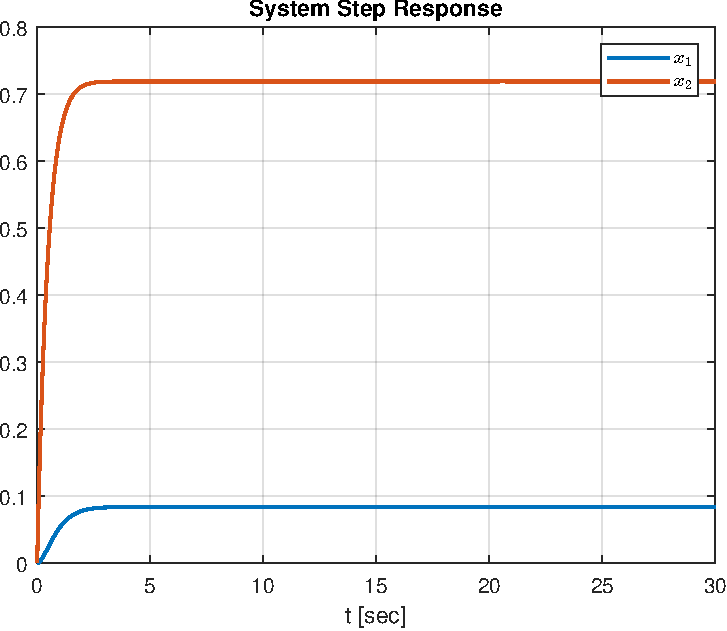
\includegraphics[width=\textwidth]{plot/task1_step_response.pdf}
    \caption{}
    \label{fig:task1_step_response}
  \end{subfigure}
  \hfill
  \begin{subfigure}[b]{0.45\textwidth}
    \centering
    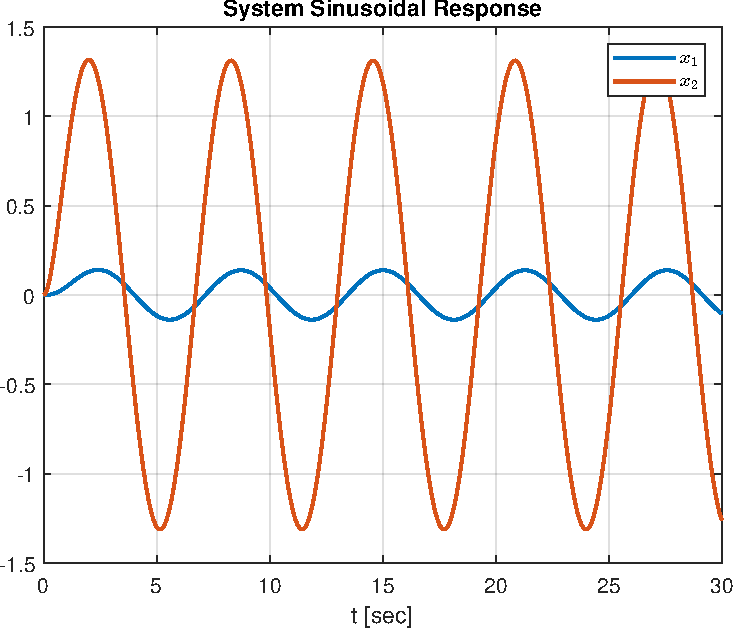
\includegraphics[width=\textwidth]{plot/task1_sinusoidal_response.pdf}
    \caption{}
    \label{fig:task1_sinusoidal_response}
  \end{subfigure}
  \caption{Απόκριση του συστήματος για α) βηματική είσοδο, β) $u(t) = 2 \sin t$}
  \label{fig:task1_response}
\end{figure}

\subsubsection*{Επιλογή εισόδου}

Για να αποτυπωθεί πλήρως η δυναμική του συστήματος, είναι σημαντικό η είσοδος να περιέχει αρκετές
συχνότητες ώστε να διεγείρει όλους τους ρυθμούς του συστήματος. Επίσης, με κατάλληλη επιλογή της
εισόδου ώστε να ικανοποιεί την Συνθήκη Εναπομείνουσας Διέγερσης (ΣΕΔ), οι μέθοδοι εκτίμησης παραμέτρων 
πραγματικού χρόνου (κλίσης, \selectlanguage{english}Lyapunov\selectlanguage{greek}) μας εγγυόνται την 
σύγκλιση των παραμετρικών σφαλμάτων στο μηδέν.

Το γραμμικό μας σύστημα είναι τάξεως $n=2$. Για να ικανοποιεί η είσοδός μας $u$ μία ΣΕΔ πρέπει
να περιέχει τουλάχιστον $m = \left\lceil \frac{n}{2} \right\rceil$ διακριτές συχνότητες και τότε
το σήμα $u$ λέγεται επιμένουσα διέγερση τάξεως $n$. Στην ανάλυσή μας παρακάτω χρησιμοποιούμε ως είσοδο
την $u(t) = 2 \sin t$.

\subsubsection*{Μέθοδος \selectlanguage{english}Lyapunov\selectlanguage{greek} με προβολή}
Λόγω της εκ των προτέρων γνώσης που έχουμε για το επιτρεπτό εύρος τιμών ορισμένων παραμέτρων, 
ο χώρος αναζήτησης $\Theta$ των παραμέτρων του μοντέλου θα περιορίζεται σε ένα υποσύνολο του $\mathbb{R}^n$.
Θα χρησιμοποιήσουμε κάποιο αναδρομικό αλγόριθμο προβολής ο οποίος εξασφαλίζει ότι οι εκτιμήσεις των
παραμέτρων παραμένουν εντός του $\Theta$. Ειδικότερα θα χρησιμοποιήσουμε τη μέθοδο 
\selectlanguage{english}Lyapunov\selectlanguage{greek} με προβολή.

Πρωτού προχωρήσουμε στην εκτίμηση των παραμέτρων, θα εξετάσουμε την ευστάθεια της μεθόδου 
\selectlanguage{english}Lyapunov\selectlanguage{greek} με Μ-δομή χωρίς περιορισμούς.

Το σύστημα αναγνώρισης είναι:
\begin{equation}
    \dot{\hat{\mathbf{x}}} = \hat{\mathbf{A}}\mathbf{x} + \hat{\mathbf{B}} u + 
    \mathbf{C}(\mathbf{x} - \hat{\mathbf{x}}),
    \label{eq:lyapunov_mixed_identification_system}
\end{equation}
όπου $\mathbf{C}$ συμμετρικός και θετικά ημιορισμένος πίνακας. Η παράγωγος του σφάλματος αναγνώρισης 
$\mathbf{e} = \mathbf{x} - \hat{\mathbf{x}}$ 
βρίσκεται:
\begin{equation}
    \dot{\mathbf{e}} = -\tilde{\mathbf{A}}\mathbf{x} - \tilde{\mathbf{B}}u - \mathbf{C}\mathbf{e}
    \label{eq:lyapunov_mixed_identification_error_derivative}
\end{equation}
όπου $\tilde{\mathbf{A}} = \hat{\mathbf{A}} - \mathbf{A}$,
$\tilde{\mathbf{B}} = \hat{\mathbf{B}} - \mathbf{B}$ τα παραμετρικά σφάλματα.
Ως συνάρτηση \selectlanguage{english}Lyapunov\selectlanguage{greek} επιλέγεται η:
\begin{equation}
    V = \frac{1}{2}\mathbf{e}^{\top}\mathbf{e} + 
    \frac{1}{2}\mathrm{Tr}\{\tilde{\mathbf{A}}^{\top}\tilde{\mathbf{A}}\}
    + \frac{1}{2}\mathrm{Tr}\{\tilde{\mathbf{B}}^{\top}\tilde{\mathbf{B}}\}
    \label{eq:lyapunov_function}
\end{equation}
Παραγωγίζοντας την (\ref{eq:lyapunov_function}) και αντικαθιστώντας
την (\ref{eq:lyapunov_mixed_identification_error_derivative}) προκύπτει:
\begin{equation}
    \dot{V} = -\mathbf{e}^{\top}\mathbf{C}\mathbf{e} + 
    \mathrm{Tr}\{\tilde{\mathbf{A}}^{\top}\dot{\hat{\mathbf{A}}} + 
    \tilde{\mathbf{B}}^{\top}\dot{\hat{\mathbf{B}}} - 
    \tilde{\mathbf{A}}\mathbf{x}\mathbf{e}^{\top} - 
    \tilde{\mathbf{B}}u\mathbf{e}^{\top}\}.
    \label{eq:lyapunov_mixed_function_derivative_1}  
\end{equation}
Επιλέγουμε:
\begin{equation}
    \begin{aligned}
        \dot{\hat{\mathbf{A}}} = \mathbf{e}\mathbf{x}^{\top} \\ 
        \dot{\hat{\mathbf{B}}} = \mathbf{e}u^{\top}
    \end{aligned}
    \label{eq:lyapunov_mixed_update_formula}
\end{equation}
και η (\ref{eq:lyapunov_mixed_function_derivative_1}) γίνεται:
\begin{equation}
    \dot{V} = -\mathbf{e}^{\top}\mathbf{C}\mathbf{e}
    \label{eq:lyapunov_mixed_function_derivative_2}
\end{equation}
Βλέπουμε ότι στη μικτή δομή ισχύει $\dot{V} \leq 0, \, \forall t$, καθώς ο $\mathbf{C}$ είναι 
συμμετρικός και θετικά ημιορισμένος. Συνεπώς, το σύστημα (\ref{eq:lyapunov_mixed_identification_system}), 
(\ref{eq:lyapunov_mixed_update_formula}) είναι ευσταθές.

Στην ανάλυσή μας θέσαμε $\mathbf{C} = k \mathbf{I}$, όπου $\mathbf{I}$ είναι ο μοναδιαίος πίνακας και 
$k > 0$ το κέρδος. Η επιλογή του $k$ έγινε με τη μέθοδο 
\selectlanguage{english}trial and error\selectlanguage{greek}. Μεγαλύτερες τιμές του $k$ έχουν ως 
αποτέλεσμα να υπερισχύει ο διορθωτικός όρος $\mathbf{C}(\mathbf{x} - \hat{\mathbf{x}})$ στην 
(\ref{eq:lyapunov_mixed_identification_system}), οδηγώντας σε ταχύτερη σύγκλιση. Ωστόσο, πολύ μεγάλες 
τιμές του $k$ ενδέχεται να καταστήσουν το σύστημα άκαμπτο. Τελικά, επιλέγουμε $k = 1$.

Έχοντας εξασφαλίσει την ευστάθεια του αλγορίθμου απουσία περιορισμών, συνεχίζουμε με την σχεδίαση του
αναδρομικού αλγορίθμου προβολής. Έστω
\[
\hat{\theta} =
\begin{bmatrix}
    \hat{\alpha}_{11} & \hat{\alpha}_{12} & \hat{\alpha}_{21} & \hat{\alpha}_{22} & \hat{b}_1 & \hat{b}_2
\end{bmatrix}^{\top}
\]
το διάνυσμα των εκτιμήσεων των παραμέτρων που προκύπτει από το σύστημα (\ref{eq:lyapunov_mixed_identification_system}), (\ref{eq:lyapunov_mixed_update_formula}). 
Θέλουμε να εξασφαλίσουμε ότι το $\hat{\theta}$ θα παίρνει τιμές εντός του κυρτού συνόλου:
\[
\Theta = \{\hat{\theta} \in \mathbb{R}^6:\, g(\hat{\theta}) \leq 0\}
\]
όπου η $g(\hat{\theta}) \in \mathbb{R}^3$ έχει διάσταση όση και το πλήθος των περιορισμών.
Από την (\ref{eq:restrictions}) έχουμε:
\[
\begin{aligned}
    \alpha_{11} \ge -3 \Rightarrow - \alpha_{11} - 3 \le 0 \\
    \alpha_{11} \le -1 \Rightarrow \alpha_{11} + 1 \le 0 \\
    b_2 \ge 1 \Rightarrow 1 - b_2 \le 0
\end{aligned}
\]
Συνεπώς η $g(\hat{\theta})$ θα είναι:
\[
    g(\hat{\theta}) = 
    \begin{bmatrix}
        - \alpha_{11} - 3 \\
        \alpha_{11} + 1 \\
        1 - b_2
    \end{bmatrix}
\]
και η Ιακωβιανή της $g(\hat{\theta})$:
\[
    \mathbf{J}_g(\hat{\theta}) = 
    \begin{bmatrix}
         \nabla g_1(\hat{\theta}) \\
         \nabla g_2(\hat{\theta}) \\
         \nabla g_3(\hat{\theta})
    \end{bmatrix} = 
    \begin{bmatrix}
        -1 & 0 & 0 & 0 & 0 & 0 \\
        1 & 0 & 0 & 0 & 0 & 0 \\
        0 & 0 & 0 & 0 & 0 & -1
    \end{bmatrix}
\]
Ο αλγόριθμος \selectlanguage{english}Lyapunov\selectlanguage{greek} με προβολή μεικτής δομής που πετυχαίνει
το παραπάνω αποτέλεσμα είναι:
\begin{equation}
    \dot{\hat{\theta}}_\Pi = 
    \begin{cases}
    \dot{\hat{\theta}}, & \text{αν } g_i(\hat{\theta}) < 0 
    \text{ ή } \nabla g_i^\top \dot{\hat{\theta}} \leq 0 \\
    \dot{\hat{\theta}} - 
    \mathbf{\Gamma} \frac{\nabla g_i {\nabla g_i}^{\top}}{{\nabla g_i}^{\top} \mathbf{\Gamma} \nabla g_i}
    \dot{\hat{\theta}}, & \text{διαφορετικά}
    \end{cases}
    \label{eq:lyapunov_mixed_projection}
\end{equation}
όπου $\mathbf{\Gamma}  = \mathbf{\Gamma}^{\top} \in \mathbb{R}^{6 \times 6}$ ο πίνακας κέρδους προσαρμογής
και ο δείκτης $i$ υποδηλώνει τον $i$-οστό περιορισμό. Ο διορθωτικός όρος 
$- \Gamma \nabla g_i \left( \nabla g_i^\top \Gamma \nabla g_i \right)^{-1} \nabla g_i^\top 
\dot{\hat{\theta}}$ εγγυάται ότι $\hat{\theta} \in \Theta, \, \forall t \ge 0$ με την προϋπόθεση ότι
$\hat{\theta}(0) \in \Theta$. Πράγματι:
\[
\begin{aligned}
\dot{\hat{\theta}}_{\Pi}^{\top} \nabla g_i &= \dot{\hat{\theta}}^{\top} \nabla g_i - 
\dot{\hat{\theta}}^{\top} \frac{\nabla g_i \nabla g_i^{\top}}{\nabla g_i^{\top} \mathbf{\Gamma} \nabla g_i}
\mathbf{\Gamma}^{\top} \nabla g_i \\
&= \dot{\hat{\theta}}^{\top} \nabla g_i - \dot{\hat{\theta}}^{\top} \nabla g_i 
\frac{\nabla g_i^{\top} \mathbf{\Gamma} \nabla g_i}{\nabla g_i^{\top} \mathbf{\Gamma} \nabla g_i} \\
&= 0
\end{aligned}
\]
Συνεπώς, όταν ο $i$-οστός περιορισμός είναι ενεργός, η γωνία μεταξύ των $\dot{\hat{\theta}}_{\Pi}^{\top}$
και $\nabla g_i$ είναι ορθή, άρα η νέα εκτίμηση $\hat{\theta}$ θα κινηθεί εφαπτομενικά πάνω στο σύνορο του 
$\Theta$.

Η ανάλυση της ευστάθειας που προηγήθηκε, αφορούσε τη μέθοδο 
\selectlanguage{english}Lyapunov\selectlanguage{greek} μεικτής δομής απουσία περιορισμών. Αποδεικνύεται 
ότι η προσθήκη του διορθωτικού όρου στην (\ref{eq:lyapunov_mixed_projection}) όχι μόνο δεν επηρεάζει 
αρνητικά την ευστάθεια του συστήματος, αλλά αντιθέτως καθιστά την παράγωγο της συνάρτησης 
\selectlanguage{english}Lyapunov\selectlanguage{greek} πιο αρνητική. Συνεπώς, τα συμπεράσματά μας περί
ευστάθειας μεταφέρονται αυτούσια και στην περίπτωση παρουσίας περιορισμών.

Στο Σχήμα~\ref{fig:task1_lyapunov} φαίνεται η γραφική παράσταση της συνάρτησης 
\selectlanguage{english}Lyapunov\selectlanguage{greek} καθώς και της παραγώγου της, για βηματική είσοδο 
(αριστερά) και ημιτονοειδή είσοδο $u(t) = 2 \sin t$ (δεξιά). Παρατηρούμε ότι και στις δύο περιπτώσεις 
ισχύει $V \geq 0, \, \dot{V} \leq 0, \forall t$, γεγονός που επιβεβαιώνει την ευστάθεια του συστήματος 
εκτίμησης παραμέτρων.

\begin{figure}[htbp]
  \centering
  \begin{subfigure}[b]{0.45\textwidth}
    \centering
    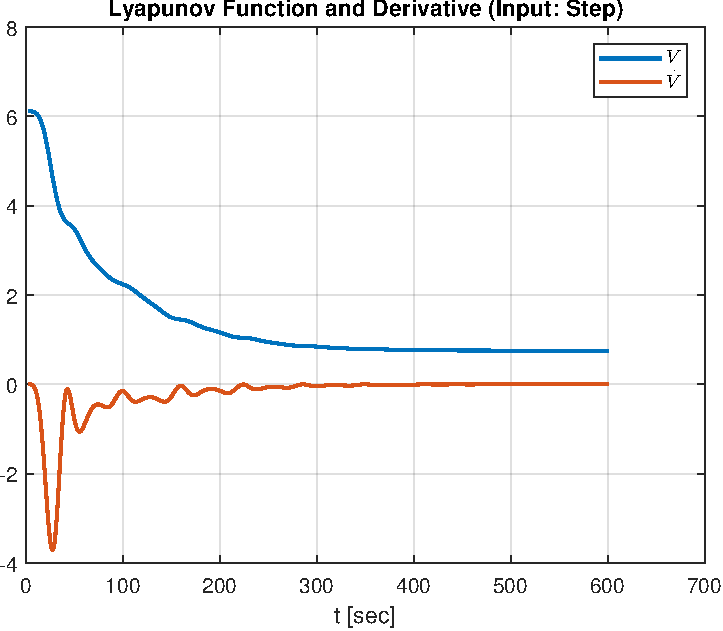
\includegraphics[width=\textwidth]{plot/task1_lyapunov_step.pdf}
    \caption{}
    \label{fig:task1_lyapunov_step}
  \end{subfigure}
  \hfill
  \begin{subfigure}[b]{0.45\textwidth}
    \centering
    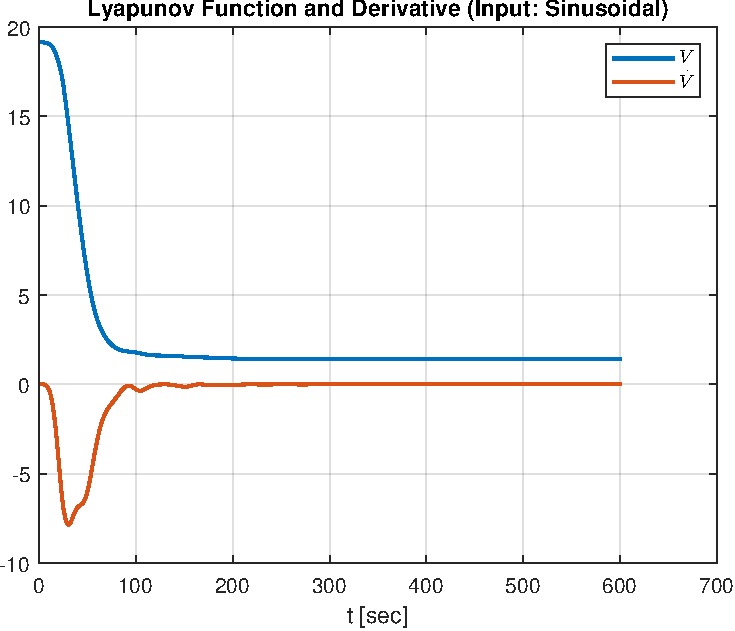
\includegraphics[width=\textwidth]{plot/task1_lyapunov_sinusoidal.pdf}
    \caption{}
    \label{fig:task1_lyapunov_sinusoidal}
  \end{subfigure}
  \caption{Γραφική παράσταση της συνάρτησης \selectlanguage{english}Lyapunov\selectlanguage{greek} καθώς και
  της παραγώγου της για α) βηματική είσοδο, β) $u(t) = 2 \sin t$}
  \label{fig:task1_lyapunov}
\end{figure}

Στο Σχήμα~\ref{fig:task1_identification_error_step} παρουσιάζεται το σφάλμα αναγνώρισης των δύο καταστάσεων 
για βηματική είσοδο, ενώ στο Σχήμα~\ref{fig:task1_identification_error_sinusoidal} απεικονίζεται το αντίστοιχο 
σφάλμα για είσοδο $u(t) = 2 \sin t$. Παρατηρούμε ότι και στις δύο περιπτώσεις τα σφάλματα συγκλίνουν στο μηδέν. 
Αυτό είναι αναμενόμενο, καθώς οι είσοδοι είναι φραγμένες και, σύμφωνα με το λήμμα 
\selectlanguage{english}Barbalat\selectlanguage{greek}, το σφάλμα αναγνώρισης τείνει στο μηδέν.

\begin{figure}
    \centering
    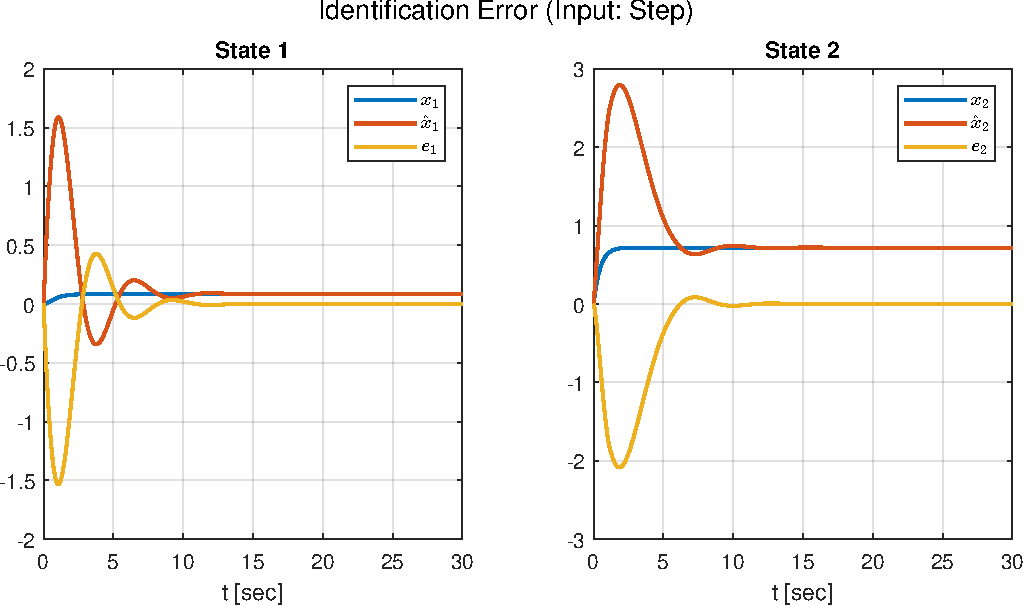
\includegraphics[width=1\linewidth]{plot/task1_identification_error_step.pdf}
    \caption{Σφάλμα αναγνώρισης για βηματική είσοδο}
    \label{fig:task1_identification_error_step}
\end{figure}

\begin{figure}
    \centering
    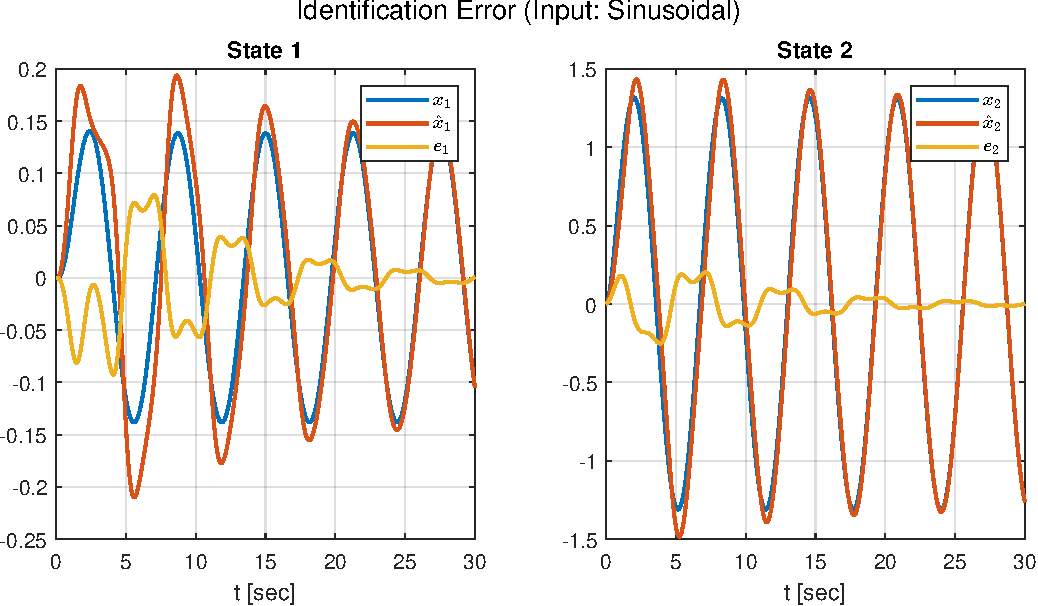
\includegraphics[width=1\linewidth]{plot/task1_identification_error_sinusoidal.pdf}
    \caption{Σφάλμα αναγνώρισης για είσοδο $u(t) = 2 \sin t$}
    \label{fig:task1_identification_error_sinusoidal}
\end{figure}

Στο Σχήμα~\ref{fig:task1_parameter_estimations} παρουσιάζονται οι εκτιμήσεις των παραμέτρων για βηματική είσοδο 
(αριστερά) και για ημιτονοειδή είσοδο $u(t) = 2 \sin t$ (δεξιά). Παρατηρούμε ότι και στις δύο περιπτώσεις 
ικανοποιούνται οι περιορισμοί $-3 \leq \hat{\alpha}_{11} \leq -1, \, b_2 \geq 1, \, \forall t$. 
Επιπλέον, για την ημιτονοειδή είσοδο όλες οι εκτιμήσεις συγκλίνουν στις πραγματικές τιμές των παραμέτρων, 
σε αντίθεση με την περίπτωση της βηματικής εισόδου. Αυτό οφείλεται στο γεγονός ότι η $u(t) = 2 \sin t$ 
ικανοποιεί τη ΣΕΔ, όπως αναλύθηκε προηγουμένως.

\begin{figure}[htbp]
  \centering
  \begin{subfigure}[b]{0.45\textwidth}
    \centering
    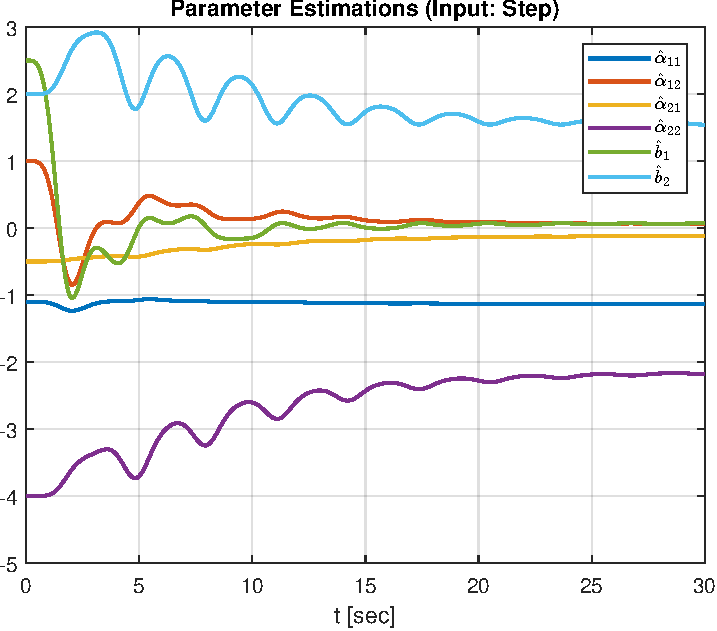
\includegraphics[width=\textwidth]{plot/task1_parameter_estimations_step.pdf}
    \caption{}
    \label{fig:task1_parameter_estimations_step}
  \end{subfigure}
  \hfill
  \begin{subfigure}[b]{0.45\textwidth}
    \centering
    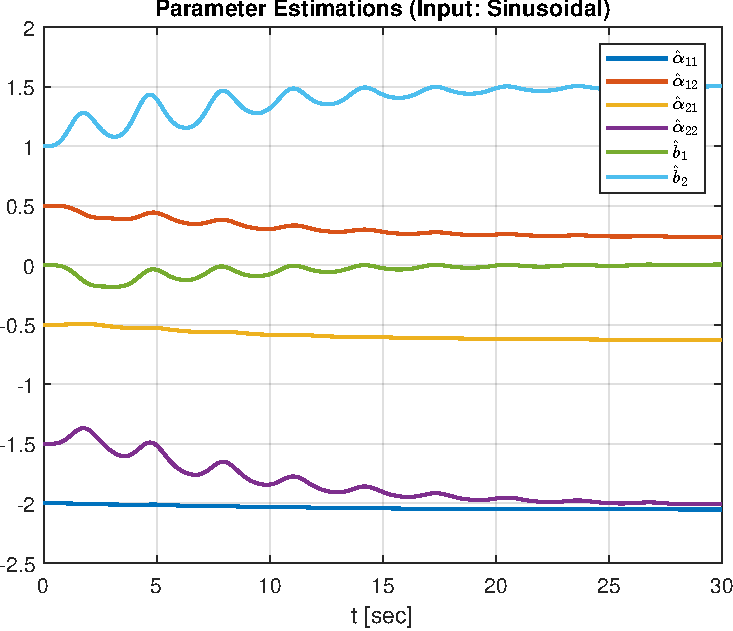
\includegraphics[width=\textwidth]{plot/task1_parameter_estimations_sinusoidal.pdf}
    \caption{}
    \label{fig:task1_parameter_estimations_sinusoidal}
  \end{subfigure}
  \caption{Εκτιμήσεις παραμέτρων για α) βηματική είσοδο, β) $u(t) = 2 \sin t$}
  \label{fig:task1_parameter_estimations}
\end{figure}


\subsection*{Εκτίμηση Παραμέτρων Παρουσία Σφάλματος Πόλωσης}
Θεωρούμε τώρα ότι στο σύστημά μας υπάρχει σφάλμα πόλωσης $\omega \in \mathbb{R}^2$ που να ικανοποιεί
$||\omega(t)|| \leq \bar{\omega}, \forall t \geq 0$, για κάποια άγνωστη σταθερά $\bar{\omega} > 0$.
Τα σφάλματα πόλωσης αποτελούν σταθερές ή αργά μεταβαλλόμενες διαταραχές που οφείλονται στην εσφαλμένη 
επιλογή της δομής του μοντέλου. Στην παρακάτω ανάλυση το σφάλμα πόλωσης μοντελοποιείται ως:
\begin{equation}
    \omega(t) = 
    \begin{bmatrix}
        \omega_1(t) \\
        \omega_2(t)
    \end{bmatrix} = 
    \begin{bmatrix}
        \bar{\omega} \sin(2 \pi f_w t) \\
        \bar{\omega} \cos(2 \pi f_w t)
    \end{bmatrix}, \quad t \geq 0
    \label{eq:bias_error}
\end{equation}
όπου $f_w << f_n$ με $f_n = \frac{\omega_n}{2 \pi}$ τη φυσική συχνότητα του συστήματος.

Παρουσία σφάλματος πόλωσης, οι κλασικές μέθοδοι εκτίμησης παραμέτρων πραγματικού χρόνου διασφαλίζουν ότι 
το σφάλμα αναγνώρισης $e$ παραμένει φραγμένο, δηλαδή $||e|| \leq \bar{\omega}$. Ωστόσο, η εκτίμηση των
παραμέτρων $\hat{\theta}$ ενδέχεται να αποκλίνει σημαντικά από τις πραγματικές τιμές $\theta^*$, 
οδηγώντας σε παραμετρικό σφάλμα $||\tilde{\theta}|| = ||\hat{\theta} - \theta|| \to \infty$.

Ένας τρόπος αντιμετώπισης της απόκλισης αυτής είναι η χρήση της μεθόδου προβολής, η οποία περιορίζει το 
διάνυσμα εκτίμησης εντός ενός κυρτού συνόλου $\Theta$, υπό την προϋπόθεση ότι $\theta^* \in \Theta$. 
Με αυτόν τον τρόπο διασφαλίζεται ότι $\hat{\theta} \in \Theta, \forall t \ge 0$, αποφεύγοντας την περίπτωση 
όπου $\hat{\theta} \to \infty$ δηλαδή την \textit{παραμετρική ολίσθηση}.

Αντί της μεθόδου προβολής, θα χρησιμοποιήσουμε έναν εύρωστο αλγόριθμο εκτίμησης παραμέτρων: 
τη μέθοδο κλίσης με διακοπτική $\sigma$-τροποποίηση.

\subsubsection*{Μέθοδος κλίσης με διακοπτική $\sigma$-τροποποίηση}

Θα φέρουμε το σύστημα της σχέσης (\ref{eq:state_space_form}) στην ισοδύναμη γραμμική παραμετροποιήσιμη 
μορφή. Από την πρώτη εξίσωση κατάστασης έχουμε:
\begin{equation}
    \dot{x}_1 = \alpha_{11} x_1 + \alpha_{12} x_2 + b_1 u
    \label{eq:linearly_parametrized_form_1}
\end{equation}
Εφόσον το $\dot{x}_1$ δεν είναι μετρήσιμο, χρησιμοποιούμε την προσέγγιση $\dot{x}_1 = s x_1$, οπότε η
(\ref{eq:linearly_parametrized_form_1}) γίνεται:
\begin{equation}
    \begin{aligned}
        &s x_1 = \alpha_{11} x_1 + \alpha_{12} x_2 + b_1 u \Rightarrow \\ 
        &(s - \alpha_{11}) x_1 = \alpha_{12} x_2 + b_1 u
    \end{aligned}
    \label{eq:linearly_parametrized_form_2}
\end{equation}
Φιλτράροντας τα δύο μέλη της (\ref{eq:linearly_parametrized_form_2}) με ευσταθές φίλτρο 1ης τάξης
$\Lambda(s) = s + \lambda, \, \lambda > 0$ παίρνουμε:
\begin{equation*}
    \begin{aligned}
        &\frac{s - \alpha_{11}}{\Lambda(s)} x_1 = \alpha_{12} \frac{x_2}{\Lambda(s)} + 
        b_1 \frac{u}{\Lambda(s)} \Rightarrow \\
        &\frac{\Lambda(s) - \lambda - \alpha_{11}}{\Lambda(s)} x_1 = \alpha_{12} \frac{x_2}{\Lambda(s)} + 
        b_1 \frac{u}{\Lambda(s)} \Rightarrow \\
        &\left(1 - \frac{\lambda + \alpha_{11}}{\Lambda(s)}\right) x_1 = \alpha_{12} \frac{x_2}{\Lambda(s)} + 
        b_1 \frac{u}{\Lambda(s)} \Rightarrow \\
        &x_1 = (\lambda + \alpha_{11})\frac{x_1}{\Lambda(s)} + \alpha_{12} \frac{x_2}{\Lambda(s)} + 
        b_1 \frac{u}{\Lambda(s)} \Rightarrow \\
        x_1 &=
        \begin{bmatrix}
            \lambda + \alpha_{11} & \alpha_{12} & b_1
        \end{bmatrix} \cdot
        \begin{bmatrix}
            \frac{x_1}{\Lambda(s)} & \frac{x_2}{\Lambda(s)} & \frac{u}{\Lambda(s)}
        \end{bmatrix}^{\top} \Rightarrow \\
        x_1 &= {\theta_1^*}^{\top} \phi
    \end{aligned} 
\end{equation*}
όπου
\begin{equation}
    \phi = 
    \begin{bmatrix}
        \frac{x_1}{\Lambda(s)} & \frac{x_2}{\Lambda(s)} & \frac{u}{\Lambda(s)}
    \end{bmatrix}^{\top}
    \label{eq:regresson_vector}
\end{equation}
το μετρήσιμο διάνυσμα οπισθοδρόμησης και
\begin{equation}
    \theta_1^* = 
    \begin{bmatrix}
        \lambda + \alpha_{11} & \alpha_{12} & b_1
    \end{bmatrix}^{\top}
    \label{eq:theta_star_1}
\end{equation}
το άγνωστο σταθερό διάνυσμα που εμπεριέχει τις πραγματικές τιμές των παραμέτρων προς εκτίμηση.

Εργαζόμενοι αντίστοιχα και για τη δεύτερη εξίσωση κατάστασης, καταλήγουμε στη γραμμικά 
παραμετροποιήσιμη μορφή:
\[
    x_2 = {\theta_2^*}^{\top} \phi
\]
με
\begin{equation}
    \theta_2^* = 
    \begin{bmatrix}
        \alpha_{21} & \lambda + \alpha_{22} & b_2
    \end{bmatrix}^{\top}
    \label{eq:theta_star_2}
\end{equation}

Οι εκτιμήσεις $\hat{\theta}_1, \, \hat{\theta}_2$ των $\theta_1^*, \, \theta_2^*$ της μεθόδου κλίσης με
διακοπτική $\sigma$-τροποποίηση (στη συνεχή της μορφή) δίνονται από τη λύση του συστήματος:
\begin{equation}
    \begin{aligned}
    x_i &= {\theta_i^*}^{\top} \phi + \omega_i, \quad |\theta_i^*| \leq M \\
    \hat{x}_i &= \hat{\theta}_i \phi \\
    \dot{\hat{\theta}}_i &= - \gamma \sigma_{\delta}(\hat{\theta}_i) \hat{\theta}_i + 
    \gamma e_i \phi, \quad \gamma > 0 \\
    e_i &= x_i - \hat{x}_i
    \end{aligned}, \quad i = 1, 2
    \label{eq:gradient_switching_sigma_modification}
\end{equation}
όπου τα σφάλματα πόλωσης $\omega_i$ δίνονται από την (\ref{eq:bias_error}), $\hat{\theta}_i$ η εκτίμηση
του $\theta_i^*$, $M, \, \bar{\sigma}, \, \gamma > 0$ σχεδιαστικές σταθερές και
\begin{equation*}
    \sigma_{\delta}(\hat{\theta}) = 
    \left\{
    \begin{aligned}
        0&, \quad \texttt{αν } ||\hat{\theta}|| < M \\
        \bar{\sigma}\left(\frac{||\hat{\theta}||}{M} - 1\right)&, 
        \quad \texttt{αν } M \leq ||\hat{\theta}|| \leq 2M \\
        \bar{\sigma}&, \quad \texttt{αν } ||\hat{\theta}|| > 2M
    \end{aligned}, \quad \bar{\sigma} > 0
    \right.
\end{equation*}

Αποδεικνύεται ότι η διακοπτική $\sigma$-τροποποίηση λύνει το πρόβλημα της παραμετρικής ολίσθησης, 
ενώ το σφάλμα αναγνώρισης συγκλίνει στο μηδέν. Ειδικότερα, για την βαθμωτή περίπτωση το παραμετρικό 
σφάλμα $\tilde{\theta} = \hat{\theta} - \theta^*$ συγκλίνει εκθετικά με ρυθμό 
$\alpha, \,0 \leq \alpha \leq \sigma_s \gamma $ στο σύνολο $\Theta$, όπου:
\begin{equation}
    \Theta = \left\{ \tilde{\theta} \in \mathbb{R}: \quad |\tilde{\theta}|^2 \leq 
    \frac{\gamma}{\alpha}\left(\bar{\omega}^2 + \sigma_s |\theta^*|^2\right)\right\}
    \label{eq:switching_sigma_parameter_estimation_bound}
\end{equation}

Από τη σχέση (\ref{eq:switching_sigma_parameter_estimation_bound}) προκύπτουν ορισμένα ιδιαίτερα 
χρήσιμα συμπεράσματα, τα οποία γενικεύονται και στην περίπτωση όπου το $\theta^*$ είναι διάνυσμα. 
Πρώτον, το άνω φράγμα του $|\tilde{\theta}|^2$ αυξάνεται με το πλάτος του σφάλματος πόλωσης 
$\bar{\omega}$. Το γεγονός αυτό επιβεβαιώνεται και από το Σχήμα~\ref{fig:task1_mse_vs_bias_error_amplitude},
στο οποίο παρατηρούμε ότι το μέσο τετραγωνικό σφάλμα 
(\selectlanguage{english}Mean Squared Error -- MSE\selectlanguage{greek}) των εκτιμήσεων των παραμέτρων 
αυξάνεται όσο αυξάνεται το $\bar{\omega}$. Αντίστοιχη είναι και η επίδραση της παραμέτρου $\gamma$ ως 
προς τη μέγιστη τιμή του παραμετρικού σφάλματος, όπως εύκολα διαπιστώνουμε από την
(\ref{eq:switching_sigma_parameter_estimation_bound}). Πράγματι, από το 
Σχήμα~\ref{fig:task1_mse_vs_gamma_gain}, φαίνεται ότι το \selectlanguage{english}MSE\selectlanguage{greek} 
των εκτιμήσεων των παραμέτρων αυξάνεται καθώς αυξάνεται η τιμή του $\gamma$.


\begin{figure}[htbp]
  \centering
  \begin{subfigure}[b]{0.45\textwidth}
    \centering
    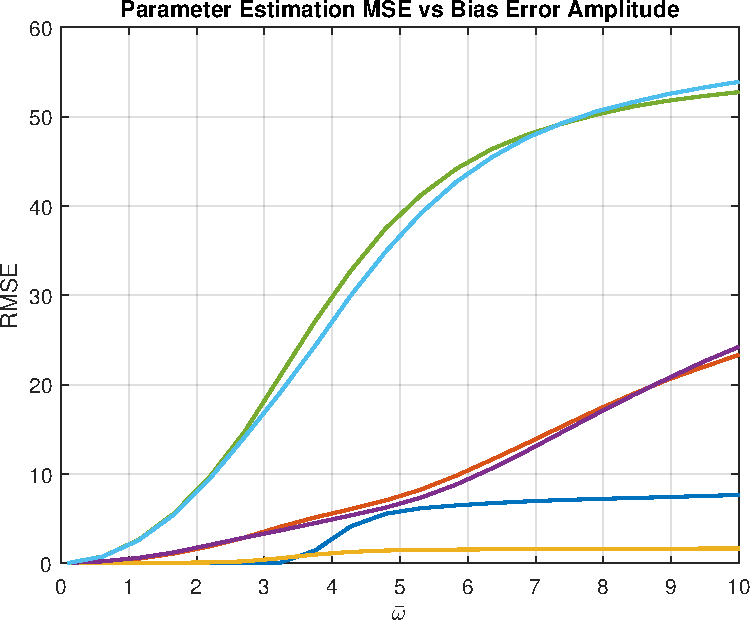
\includegraphics[width=\textwidth]{plot/task1_mse_vs_bias_error_amplitude.pdf}
    \caption{}
    \label{fig:task1_mse_vs_bias_error_amplitude}
  \end{subfigure}
  \hfill
  \begin{subfigure}[b]{0.45\textwidth}
    \centering
    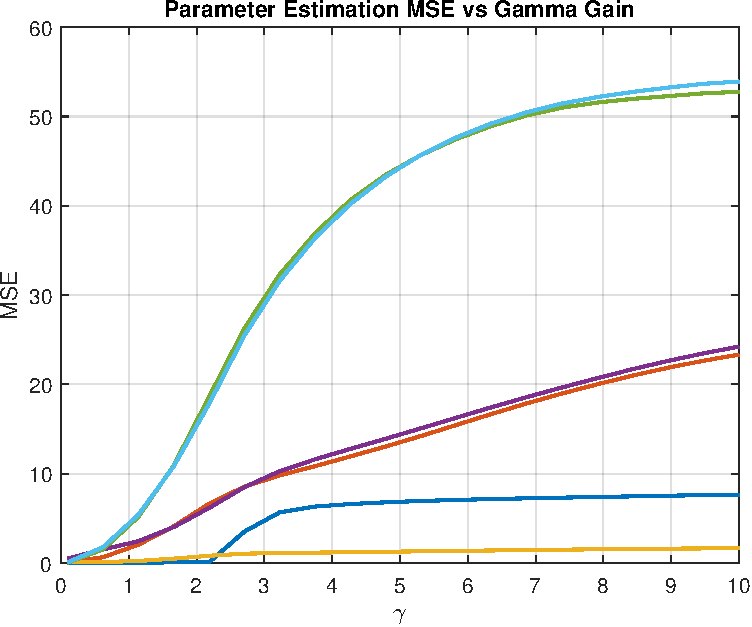
\includegraphics[width=\textwidth]{plot/task1_mse_vs_gamma_gain.pdf}
    \caption{}
    \label{fig:task1_mse_vs_gamma_gain}
  \end{subfigure}
  \caption{Γραφική παράσταση του \selectlanguage{english}MSE\selectlanguage{greek} των εκτιμήσεων των
    παραμέτρων ως προς α) το πλάτος του θορύβου $\bar{\omega}$ β) το κέρδος $\gamma$}
  \label{fig:task1_mse_vs_design_parameters}
\end{figure}

Οι σχεδιαστικές σταθερές $M, \, \bar{\sigma}, \, \gamma > 0$ επιλέχθηκαν με τη μέθοδο
\selectlanguage{english}trial and error\selectlanguage{greek}.
Ειδικότερα, το $M$ επιλέγεται ώστε να ισχύει η απαίτηση $|\theta_i^*| \leq M$. Όσο πιο μεγάλο είναι το $M$,
τόσο ``καθυστερεί'' η εφαρμογή της $\sigma$-τροποποίησης, άρα τόσο επιτρέπεται στο $\hat{\theta}_i$ να ολισθήσει
σε μεγαλύτερες τιμές μέχρι να ``ενεργοποιηθεί'' η $\sigma$-τροποποίηση. Ο συντελεστής $\gamma$ ελέγχει 
-- πέρα από το μέγιστο παραμετρικό σφάλμα, όπως ήδη έχουμε αναφέρει -- την ταχύτητα σύγκλισης του 
$\hat{x}_i(t)$ στο $x_i(t)$. Αυξάνοντας την τιμή του $\gamma$ επιτυγχάνεται ταχύτερη σύγκλιση. Πολύ μεγάλες 
τιμές του $\gamma$ όμως καθιστούν το σύστημά μας ``άκαμπτο''. Τέλος, η παράμετρος $\bar{\sigma}$ ορίζει το 
πόσο βίαια ``τραβάει'' η μέθοδος τις εκτιμήσεις των παραμέτρων όταν απομακρύνονται από το κατώφλι $M$. Τελικά
επιλέγουμε $M = 10, \, \bar{\sigma} = 5, \, \gamma = 10$.

Στο Σχήμα~\ref{fig:task1_gradient_parameter_estimations} παρουσιάζονται οι εκτιμήσεις των παραμέτρων για 
την προαναφερθείσα επιλογή των σχεδιαστικών σταθερών. Παρατηρείται ότι οι εκτιμήσεις εμφανίζουν ταλαντώσεις
πεπερασμένου πλάτους γύρω από τις πραγματικές τιμές των παραμέτρων. Το φαινόμενο αυτό συνάδει με τα 
συμπεράσματα που προέκυψαν από τη σχέση (\ref{eq:switching_sigma_parameter_estimation_bound}), σύμφωνα με 
την οποία το παραμετρικό σφάλμα παραμένει φραγμένο.

\begin{figure}
    \centering
    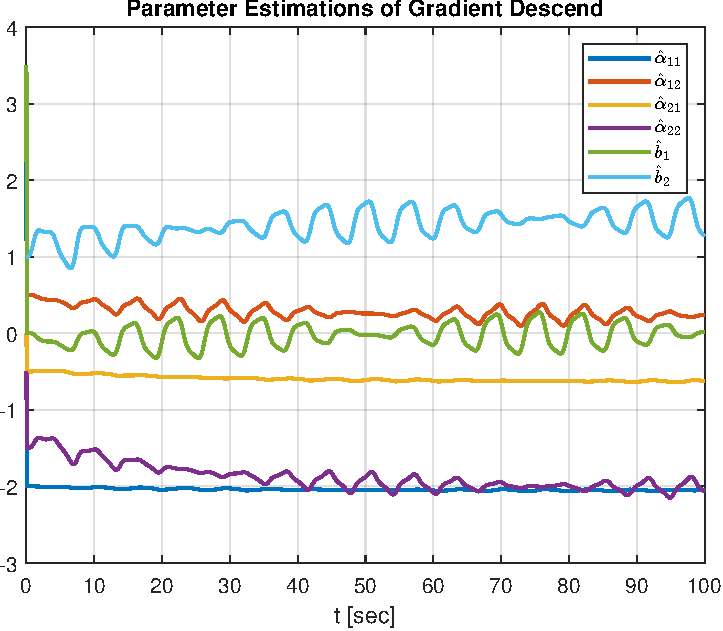
\includegraphics[width=0.5\linewidth]{plot/task1_gradient_parameter_estimations.pdf}
    \caption{Εκτιμήσεις παραμέτρων της μεθόδου κλίσης με διακοπτική $\sigma$-τροποποίηση}
    \label{fig:task1_gradient_parameter_estimations}
\end{figure}

Τέλος, στο Σχήμα~\ref{fig:task1_gradient_identification_error} φαίνεται το σφάλμα αναγνώρισης των δύο 
καταστάσεων του συστήματος.

\begin{figure}
    \centering
    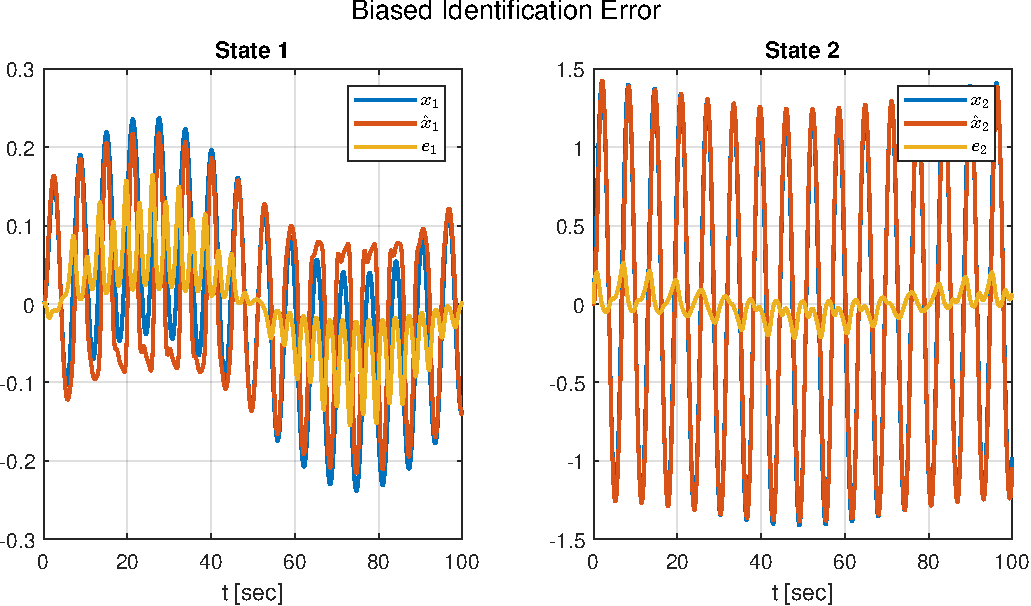
\includegraphics[width=1\linewidth]{plot/task1_gradient_identification_error.pdf}
    \caption{Σφάλματα αναγνώρισης της μεθόδου κλίσης με διακοπτική $\sigma$-τροποποίηση}
    \label{fig:task1_gradient_identification_error}
\end{figure}

\newpage

\section*{Θέμα 2}
Σε αυτό το μέρος καλούμαστε να μοντελοποιήσουμε και στη συνέχεια να αξιολογήσουμε ένα άγνωστο μη-γραμμικό 
δυναμικό σύστημα της μορφής:
\[
    \dot{x} = f(x(t), \, u(t), \, \theta),
\]
όπου $f:\, \mathbb{R}^2 \to \mathbb{R}$ είναι μία άγνωστη μη-γραμμική συνάρτηση, $x(t)$ η έξοδος του 
συστήματος και $u(t)$ η είσοδος, οι οποίες θεωρούνται μετρήσιμες, και 
$\theta = [\theta_1 \quad \theta_2]^{\top}$ είναι ένα σταθερό διάνυσμα παραμέτρων με 
$\theta_1, \, \theta_2 \in [0.5, \, 2]$. Για την προσομοίωση της απόκρισης του πραγματικού συστήματος
θεωρούμε ότι $f(x, u, \theta) = -x^3 + \theta_1 \tanh(x) + \theta_2 \frac{1}{1 + x^2} + u$
και επιλέγουμε $\theta = [1.2, \, 0.8]^{\top}$.

\subsection*{Ερώτημα α)}

\subsubsection*{Επιλογή δομής μοντέλου}
Δεδομένου ότι δεν έχουμε καμία εκ των προτέρων πληροφορία για τη μορφή του υπό μελέτη συστήματος, η προσέγγιση
που ακολουθούμε ανήκει στην κατηγορία ``μαύρο κουτί''. Το πρώτο βήμα σε μια τέτοια προσέγγιση είναι η επιλογή 
της δομής του μοντέλου, δηλαδή της μαθηματικής του περιγραφής. Υποθέτουμε ότι το μοντέλο περιγράφεται από τη 
γραμμικά παραμετροποιήσιμη μορφή:
\[
    y = {\theta^*}^{\top} \phi,
\]
όπου:
\[
    \phi = 
    \begin{bmatrix}
        g_1(x) & g_2(x) & \cdots & g_N(x)
    \end{bmatrix}^{\top}
\]
είναι το διάνυσμα οπισθοδρόμησης, $g_i(x): \, \mathbb{R} \to \mathbb{R}, \, i = 1,\dots,N$ οι συναρτήσεις 
βάσης, και $\theta^* \in \mathbb{R}^N$ το διάνυσμα των συντελεστών. Οι συναρτήσεις βάσης που εξετάζονται 
είναι:
\begin{itemize}
    \item \textbf{Πολυωνυμικές:} $g_i(x) = x^i, \, i = 1,\dots,N$
    \item \textbf{Γκαουσιανού πυρήνα:} $g_i(x) = e^{-(x - c_i)^2 / (2 w_i^2)}, \quad c_i \neq c_j, \quad i \neq j$
    \item \textbf{Ημιτονοειδείς:} $g_i(x) = \sin(w_i t), \quad w_i \neq w_j, \quad i \neq j$
\end{itemize}

Ένα δεύτερο κρίσιμο ζήτημα, μετά την επιλογή της μορφής του μοντέλου, είναι ο προσδιορισμός της 
πολυπλοκότητας του, δηλαδή του πλήθους των παραμέτρων $N$, που ισοδυναμεί με τη διάσταση του διανύσματος 
$\theta^*$. Μία κοινή τεχνική επιλογής του πλήθους των παραμέτρων είναι η \textbf{προσθετική δόμηση}, η 
οποία ανήκει στις \textit{άμεσες τεχνικές} επιλογής δομής. Σύμφωνα με αυτή τη μεθοδολογία, ξεκινάμε από 
ένα απλό μοντέλο και αυξάνουμε προοδευτικά την πολυπλοκότητά του προσθέτοντας παραμέτρους. Ως κατάλληλο 
πλήθος παραμέτρων $n^*$ επιλέγεται αυτό που ελαχιστοποιεί το σφάλμα μοντελοποίησης. Η επιλογή αυτή δεν 
είναι απαραίτητα η βέλτιστη συνολικά, αλλά είναι η βέλτιστη εντός της εξεταζόμενης οικογένειας μοντέλων.

Στο Σχήμα~\ref{fig:task2_modeling_error_vs_model_complexity} παρουσιάζεται η εφαρμογή της προσθετικής δόμησης 
και για τις τρεις οικογένειες μοντέλων που προκύπτουν από τις υπό μελέτη συναρτήσεις βάσης. Ειδικότερα, το 
σύνολο των δεδομένων χωρίστηκε σε υποσύνολα εκπαίδευσης και ελέγχου. Σε κάθε επανάληψη, η εκτίμηση των 
παραμέτρων έγινε με βάση το σύνολο εκπαίδευσης, ενώ η αξιολόγηση του μοντέλου πραγματοποιήθηκε στο σύνολο
ελέγχου.

Από το Σχήμα~\ref{fig:task2_modeling_error_vs_model_complexity} προκύπτουν ορισμένα ιδιαίτερα χρήσιμα
συμπεράσματα. Παρατηρούμε ότι, ανεξαρτήτως της επιλεγμένης δομής του μοντέλου, το σφάλμα εκπαίδευσης 
μειώνεται μονοτονικά καθώς αυξάνεται το πλήθος των παραμέτρων $n$. Ωστόσο, η ίδια συμπεριφορά δεν 
παρατηρείται στο σφάλμα ελέγχου.

Όταν το $n$ είναι μικρό, το σφάλμα ελέγχου διατηρείται σε υψηλά επίπεδα, γεγονός που υποδηλώνει 
\textit{υποεκμάθηση} (\selectlanguage{english}underfitting\selectlanguage{greek}) -- δηλαδή, το μοντέλο 
δεν είναι αρκετά ευέλικτο ώστε να συλλάβει τη δυναμική του συστήματος. Καθώς αυξάνεται το $n$, το 
μοντέλο προσαρμόζεται καλύτερα στα δεδομένα και το σφάλμα ελέγχου μειώνεται.

Ωστόσο, πέρα από μια συγκεκριμένη τιμή του $n$, η περαιτέρω αύξηση των παραμέτρων οδηγεί σε μείωση της 
απόδοσης στο σύνολο ελέγχου. Το σφάλμα αρχίζει να αυξάνεται ξανά, και για πολύ μεγάλες τιμές του $n$ 
γίνεται ιδιαίτερα υψηλό. Αυτό είναι ένδειξη \textit{υπερεκμάθησης} 
(\selectlanguage{english}overfitting\selectlanguage{greek}) -- το μοντέλο απομνημονεύει τα 
δεδομένα εκπαίδευσης, αλλά αποτυγχάνει να γενικεύσει σε νέα δεδομένα.

Η παρατήρηση αυτή επιβεβαιώνει την ανάγκη ύπαρξης ενός κατάλληλου συμβιβασμού μεταξύ πολυπλοκότητας 
μοντέλου και ικανότητας γενίκευσης, γεγονός που καθιστά την επιλογή του κατάλληλου πλήθους παραμέτρων 
$n$ κομβικής σημασίας.

Τονίζουμε ότι το σφάλμα μοντελοποίησης εκτιμάται αποκλειστικά με βάση τα δεδομένα ελέγχου και όχι τα 
δεδομένα εκπαίδευσης. Εάν δεν είχαμε προβεί σε αυτόν τον διαχωρισμό, θα οδηγούμασταν στην εσφαλμένη 
εντύπωση ότι η συνεχής μείωση του σφάλματος με την αύξηση του πλήθους των παραμέτρων $n$ αντανακλά 
βελτίωση της ικανότητας μοντελοποίησης. Στην πραγματικότητα, η μείωση αυτή αφορά το \textit{σφάλμα πόλωσης}, 
δηλαδή τη μεροληψία που προκύπτει λόγω ανεπαρκούς ή ακατάλληλης επιλογής δομής μοντέλου. Η χρήση μόνο των 
δεδομένων εκπαίδευσης μπορεί να αποκρύψει το φαινόμενο της υπερεκμάθησης και να οδηγήσει σε λανθασμένα 
συμπεράσματα ως προς την αποδοτικότητα του μοντέλου.

Συνοψίζοντας, το βέλτιστο πλήθος παραμέτρων που προκύπτει από το γράφημα είναι $n^* = 2, \, 3, \, 3$
για τις οικογένειες πολυωνυμικών, ημιτονοειδών και γκαουσιανών συναρτήσεων βάσης αντίστοιχα.

\begin{figure}
    \centering
    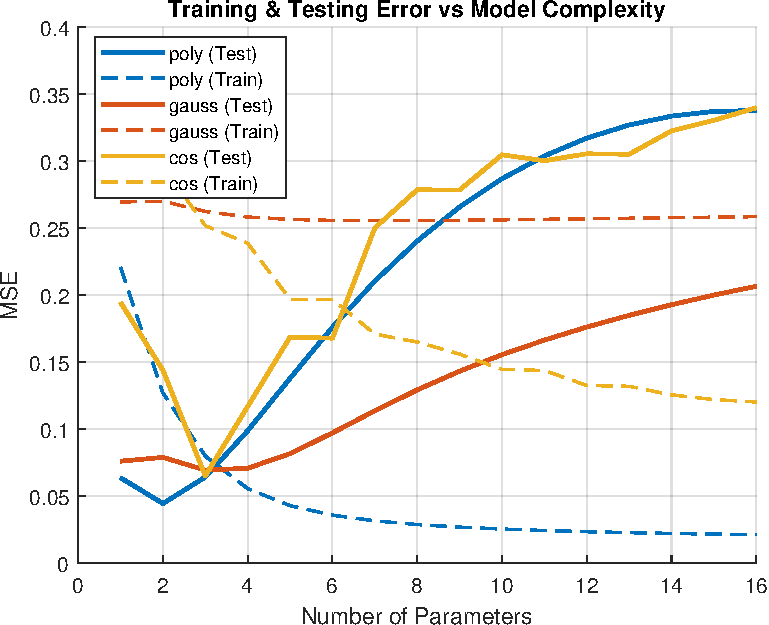
\includegraphics[width=0.5\linewidth]{plot/task2_modeling_error_vs_model_complexity.pdf}
    \caption{Σφάλμα μοντελοποίησης συναρτήσει του πλήθους των παραμέτρων του μοντέλου}
    \label{fig:task2_modeling_error_vs_model_complexity}
\end{figure}

\subsubsection*{Αξιολόγηση μοντέλου}
Έχοντας επιλέξει τη δομή και την πολυπλοκότητα των τριών υποψήφιων μοντέλων, προχωράμε στην αξιολόγησή 
τους, δηλαδή στον έλεγχο του κατά πόσο περιγράφουν επαρκώς τη συμπεριφορά του πραγματικού συστήματος. 
Από την προηγούμενη ανάλυση έχει καταστεί σαφές ότι η ποιότητα ενός μοντέλου εκτιμάται με ακρίβεια μόνο 
όταν αξιολογείται σε δεδομένα που δεν χρησιμοποιήθηκαν κατά τη φάση της εκπαίδευσης.

Ένας συνήθης και ιδιαίτερα χρήσιμος τρόπος αξιολόγησης -- ιδίως όταν το πλήθος των διαθέσιμων δεδομένων 
είναι περιορισμένο -- είναι η διαδικασία της \textit{εγκάρσιας αξιολόγησης} 
(\selectlanguage{english}cross validation\selectlanguage{greek}).

Η εγκάρσια αξιολόγηση λειτουργεί με το να χωρίζει τα δεδομένα σε $K$ ίσα υποσύνολα 
(\selectlanguage{english}``folds''\selectlanguage{greek}). Το μοντέλο εκπαιδεύεται κάθε φορά σε $K-1$ 
υποσύνολα και αξιολογείται στο εναπομείναν, με τη διαδικασία να επαναλαμβάνεται ώστε κάθε υποσύνολο να 
λειτουργήσει μία φορά ως σύνολο ελέγχου. Ο μέσος όρος του σφάλματος σε όλα τα 
\selectlanguage{english}folds\selectlanguage{greek} αποτελεί την τελική εκτίμηση της γενικευτικής 
ικανότητας του μοντέλου.

Για την εκπαίδευση των μοντέλων χρησιμοποιήθηκε η μέθοδος κλίσης με διακοπτική 
$\sigma$-τροποποίηση, όπως δίνεται στη σχέση~(\ref{eq:gradient_switching_sigma_modification}), 
καθώς εξετάζουμε τη μη ιδανική περίπτωση όπου η παρουσία σφάλματος πόλωσης είναι αναπόφευκτη.

Εφόσον για την εκτίμηση των παραμέτρων χρησιμοποιείται αλγόριθμος πραγματικού χρόνου, η χρονική αλληλουχία
των δεδομένων έχει σημασία. Όταν το \selectlanguage{english}fold\selectlanguage{greek} αξιολόγησης είναι
ενδιάμεσο, τα δεδομένα εκπαίδευσης διασπώνται, δημιουργώντας μία ασυνέχεια που δεν είναι αντιπροσωπευτική
του πραγματικού συστήματος. Συνεπώς, υιοθετούμε μία παραλλαγή της τυπικής εγκάρσιας αξιολόγησης, στην οποία 
τα δεδομένα εισόδου-εξόδου κάθε \selectlanguage{english}fold\selectlanguage{greek} είναι ανεξάρτητα μεταξύ τους 
και προέρχονται από διαφορετικά σήματα εισόδου. Σε κάθε επανάληψη, επιλέγεται ένα 
\selectlanguage{english}fold\selectlanguage{greek} για την εκπαίδευση του μοντέλου, ενώ σε καθένα από τα 
υπόλοιπα $K-1$ \selectlanguage{english}folds\selectlanguage{greek} υπολογίζεται το 
\selectlanguage{english}MSE\selectlanguage{greek}. Το σφάλμα της επανάληψης αυτής υπολογίζεται ως ο μέσος όρος
των \selectlanguage{english}MSE\selectlanguage{greek} στα υπόλοιπα $K-1$ 
\selectlanguage{english}folds\selectlanguage{greek}. 

Η υλοποίηση των παραπάνω παρουσιάζεται στο Σχήμα~\ref{fig:task2_cross_validation}, για τα μοντέλα που 
επέδειξαν την καλύτερη γενίκευση σε νέα δεδομένα κατά το στάδιο επιλογής δομής μοντέλου, δηλαδή το 
πολυωνυμικό μοντέλο δεύτερης τάξης και το μοντέλο βάσεων γκαουσιανού πυρήνα τρίτης τάξης. 
Παρατηρούμε ότι ανεξαρτήτως του \selectlanguage{english}fold\selectlanguage{greek} που επιλέγεται για εκπαίδευση,
το πολυωνυμικό μοντέλο υπερτερεί του μοντέλου γκαουσιανών πυρήνων. Συνεπώς, είναι ασφαλές να συμπεράνουμε 
ότι το πολυωνυμικό μοντέλο δεύτερης τάξης είναι καταλληλότερο. Οι είσοδοι που χρησιμοποιήθηκαν σε κάθε 
\selectlanguage{english}fold\selectlanguage{greek} είναι: 
$\sin(2 \pi t), \, 1, \, \sin(2 \pi t + \sin(0.5 \pi t)), \, e^{-t} \sin(2 \pi t), \, 1 + e^{-t}$.

\begin{figure}
    \centering
    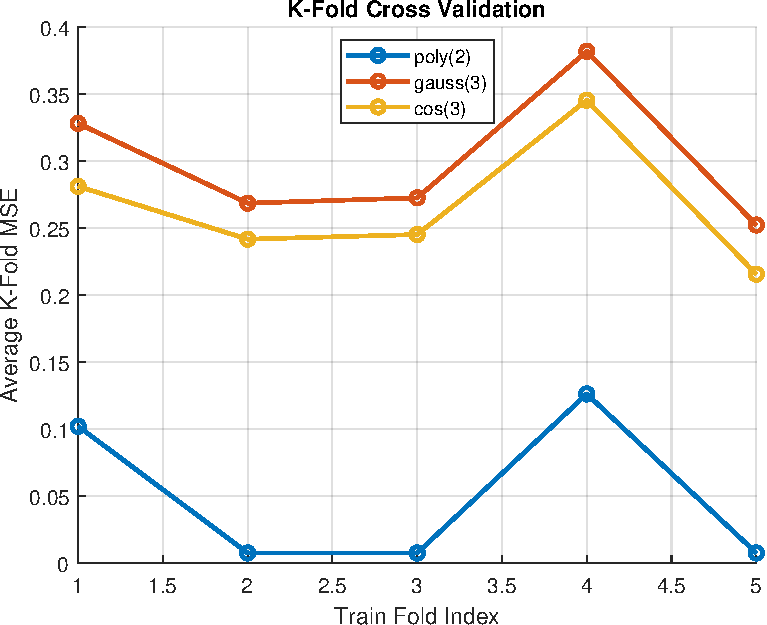
\includegraphics[width=0.5\linewidth]{plot/task2_cross_validation.pdf}
    \caption{Εγκάρσια αξιολόγηση πολυωνυμικού μοντέλου δεύτερης τάξης και μοντέλου συναρτήσεων 
    βάσης γκαουσιανού πυρήνα τρίτης τάξης}
    \label{fig:task2_cross_validation}
\end{figure}

\subsection*{Ερώτημα β)}
\subsubsection{Εύρεση τελικής μορφής μοντέλου}
Έχοντας καταλήξει στη δομή του μοντέλου, δηλαδή στο πολυωνυμικό μοντέλο δεύτερης τάξης, στόχος μας είναι
να εκτιμήσουμε το διάνυσμα παραμέτρων $\hat{\theta}$, ώστε να ελαχιστοποιείται το συνολικό σφάλμα 
μοντελοποίησης $\int_0^t e^2(\tau)d\tau$. Ακολουθώντας την ίδια μεθοδολογία όπως και κατά την επιλογή δομής
μοντέλου, διαχωρίζουμε τα δεδομένα μας σε δεδομένα εκπαίδευσης και ελέγχου. Το σφάλμα μοντελοποίησης, όπως
είδη έχουμε εξηγήσει, θα υπολογιστεί από τα δεδομένα ελέγχου. Επίσης, θεωρούμε ότι τα δεδομένα ελέγχου
προέρχονται από διαφορετικό σήμα εισόδου από αυτό των δεδομένων εκπαίδευσης. Ουσιαστικά καλούμαστε να
κάνουμε \selectlanguage{english}fine-tuning\selectlanguage{greek} στο σήμα εισόδου των δεδομένων εκπαίδευσης
καθώς και στις παραμέτρους του αλγορίθμου εκτίμησης παραμέτρων πραγματικού χρόνου ώστε να ελαχιστοποιείται
το σφάλμα μοντελοποίησης στα δεδομένα ελέγχου.

Οι είσοδοι που επιλέγουμε για να παράξουμε τα δεδομένα εκπαίδευσης είναι της μορφής:
\[
    u_K(t) = \sum_{k=1}^K \sin(2 \pi kt)
\]
ενώ για τα δεδομένα ελέγχου επιλέγουμε την βηματική είσοδο. Στο Σχήμα~\ref{} φαίνεται το αθροιστικό σφάλμα
μοντελοποίησης στα δεδομένα ελέγχου συναρτήσει του πλήθους των συχνοτήτων στο σήμα εισόδου των δεδομένων 
εκπαίδευσης.

\end{document}
